\section{Softwarearchitektur und Design}

\subsection{Grundlagen der Software-Architektur}

\begin{concept}{Grundlagen und Überblick}
\begin{itemize}
    \item \textbf{Business Analyse:}
    \begin{itemize}
        \item Domänenmodell und Kontextdiagramm
        \item Requirements (funktional und nicht-funktional)
        \item Vision und Stakeholder
    \end{itemize}
    
    \item \textbf{Architektur:}
    \begin{itemize}
        \item Logische Struktur des Systems
        \item Technische Konzeption
        \item Qualitätsanforderungen
    \end{itemize}
\end{itemize}

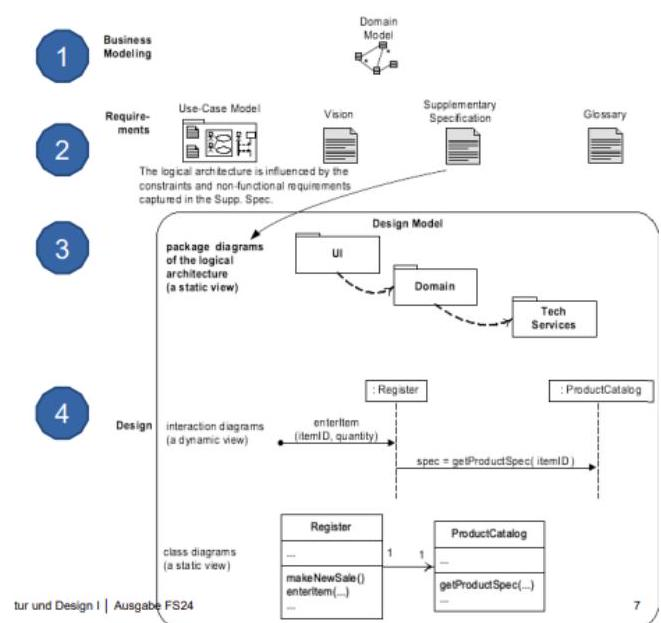
\includegraphics[width=\linewidth]{images/2024_12_29_0d1d7b5551ea1b4b41bdg-07(2)}
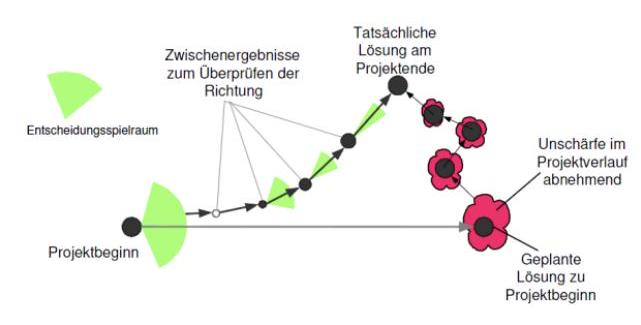
\includegraphics[width=\linewidth]{images/2024_12_29_0d1d7b5551ea1b4b41bdg-08(1)}
\end{concept}

\begin{definition}{Softwarearchitektur}
Die Architektur eines Softwaresystems definiert:
\begin{itemize}
    \item \textbf{Grundlegende Entscheidungen:}
    \begin{itemize}
        \item Programmiersprachen und Plattformen
        \item Aufteilung in Teilsysteme und Komponenten
        \item Schnittstellen zwischen Komponenten
    \end{itemize}
    
    \item \textbf{Strukturelle Aspekte:}
    \begin{itemize}
        \item Verantwortlichkeiten der Teilsysteme
        \item Abhängigkeiten zwischen Komponenten
        \item Einsatz von Basis-Technologien
    \end{itemize}
\end{itemize}
\end{definition}

\subsection{Architektur-Design}

\begin{concept}{Modulkonzept}
Ein Modul wird bewertet nach:
\begin{itemize}
    \item \textbf{Kohäsion:} Innerer Zusammenhang
    \item \textbf{Kopplung:} Externe Abhängigkeiten
\end{itemize}

\textbf{Eigenschaften:}
\begin{itemize}
    \item Autarkes Teilsystem
    \item Minimale externe Schnittstellen
    \item Enthält alle benötigten Funktionen/Daten
    \item Verschiedene Formen: Paket, Library, Service
\end{itemize}
\end{concept}

\begin{definition}{Schnittstellen}
Module kommunizieren über definierte Schnittstellen:
\begin{itemize}
    \item \textbf{Exportierte Schnittstellen:}
    \begin{itemize}
        \item Definieren angebotene Funktionalität
        \item Vertraglich garantierte Leistungen
        \item Einzige nach außen sichtbare Information
    \end{itemize}
    
    \item \textbf{Importierte Schnittstellen:}
    \begin{itemize}
        \item Von anderen Modulen benötigte Funktionalität
        \item Definieren Abhängigkeiten
        \item Basis für Kopplung
    \end{itemize}
\end{itemize}
\end{definition}

\subsection{Architektur-Prozess}

\begin{KR}{Architekturanalyse}
\textbf{1. Anforderungen sammeln}
\begin{itemize}
    \item Funktionale Anforderungen gruppieren
    \item Nicht-funktionale Anforderungen identifizieren
    \item Randbedingungen dokumentieren
\end{itemize}

\textbf{2. Qualitätsziele definieren}
\begin{itemize}
    \item Messbare Kriterien festlegen
    \item Priorisierung vornehmen
    \item Trade-offs identifizieren
\end{itemize}

\textbf{3. Einflussfaktoren analysieren}
\begin{itemize}
    \item Technische Faktoren
    \item Organisatorische Faktoren
    \item Wirtschaftliche Faktoren
\end{itemize}
\end{KR}

\begin{KR}{Architektur-Evaluation}
\textbf{1. Qualitätsattribute identifizieren}
\begin{itemize}
    \item Performance
    \item Skalierbarkeit
    \item Wartbarkeit
    \item Sicherheit
\end{itemize}

\textbf{2. Szenarien entwickeln}
\begin{itemize}
    \item Normale Nutzung
    \item Grenzfälle
    \item Fehlerfälle
    \item Wartungsszenarien
\end{itemize}

\textbf{3. Architektur analysieren}
\begin{itemize}
    \item Strukturanalyse
    \item Verhaltensanalyse
    \item Trade-off Analyse
\end{itemize}
\end{KR}

%todo: Add architectural process example

\subsection{Architektur-Muster und Clean Code}

\begin{concept}{Architekturmuster Übersicht}
Grundlegende Architekturmuster für Software-Systeme:

\begin{itemize}
    \item \textbf{Layered Pattern:} 
    \begin{itemize}
        \item Strukturierung in horizontale Schichten
        \item Klare Trennung der Verantwortlichkeiten
        \item Abhängigkeiten nur nach unten
    \end{itemize}
    
    \item \textbf{Client-Server Pattern:}
    \begin{itemize}
        \item Verteilung von Diensten
        \item Zentralisierte Ressourcen
        \item Mehrere Clients pro Server
    \end{itemize}
    
    \item \textbf{Master-Slave Pattern:}
    \begin{itemize}
        \item Verteilung von Aufgaben
        \item Zentrale Koordination
        \item Parallelverarbeitung
    \end{itemize}
    
    \item \textbf{Pipe-Filter Pattern:}
    \begin{itemize}
        \item Datenstromverarbeitung
        \item Verkettung von Operationen
        \item Wiederverwendbare Filter
    \end{itemize}
    
    \item \textbf{Event-Bus Pattern:}
    \begin{itemize}
        \item Asynchrone Kommunikation
        \item Publisher-Subscriber Modell
        \item Lose Kopplung
    \end{itemize}
\end{itemize}
%todo: Add example diagrams for each pattern
\end{concept}

\begin{concept}{Clean Architecture}
\textbf{Hauptprinzipien:}
\begin{itemize}
    \item Unabhängigkeit von Frameworks
    \item Unabhängigkeit von UI
    \item Unabhängigkeit von Datenbank
    \item Testbarkeit ohne externe Systeme
\end{itemize}

\textbf{Schichten (von innen nach außen):}
\begin{itemize}
    \item \textbf{Entities:} Zentrale Business Rules
    \item \textbf{Use Cases:} Anwendungsspezifische Business Rules
    \item \textbf{Interface Adapters:} Datenkonvertierung
    \item \textbf{Frameworks \& Drivers:} Externe Tools
\end{itemize}

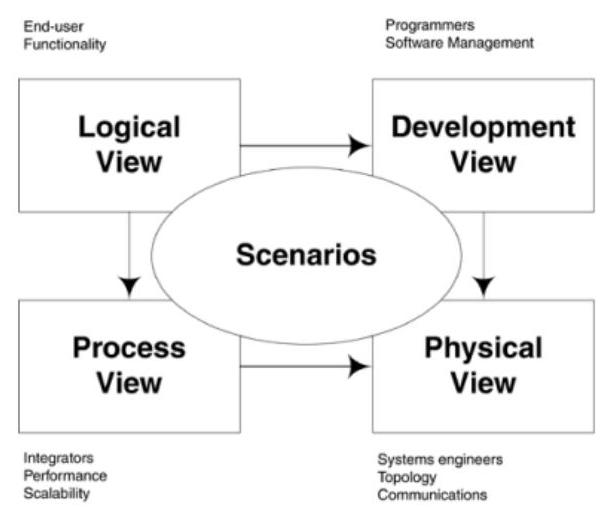
\includegraphics[width=0.9\linewidth]{images/2024_12_29_0d1d7b5551ea1b4b41bdg-09}
\end{concept}

\subsection{UML-Modellierung}

\begin{concept}{UML im Design}
UML wird in zwei Hauptaspekten verwendet:

\textbf{Statische Modelle:}
\begin{itemize}
    \item Struktur des Systems
    \item Klassendiagramme, Paketdiagramme
    \item Fokus auf Pakete, Klassen, Attribute
    \item Keine Methodenimplementierung
\end{itemize}

\textbf{Dynamische Modelle:}
\begin{itemize}
    \item Verhalten des Systems
    \item Sequenz-, Zustands-, Aktivitätsdiagramme
    \item Fokus auf Logik und Verhalten
    \item Methodenimplementierung
\end{itemize}
\end{concept}

\begin{KR}{UML Diagrammauswahl}
\textbf{1. Statische Struktur}
\begin{itemize}
    \item Klassendiagramm für Typen und Beziehungen
    \item Paketdiagramm für Modularisierung
    \item Komponentendiagramm für Bausteinsicht
    \item Verteilungsdiagramm für physische Verteilung
\end{itemize}

\textbf{2. Dynamisches Verhalten}
\begin{itemize}
    \item Sequenzdiagramm für zeitliche Abläufe
    \item Kommunikationsdiagramm für Objektkollaborationen
    \item Zustandsdiagramm für Objektlebenszyklen
    \item Aktivitätsdiagramm für Geschäftsprozesse
\end{itemize}

\textbf{3. Verwendungszweck}
\begin{itemize}
    \item Analyse: Konzeptuelle Modellierung
    \item Design: Detaillierte Spezifikation
    \item Implementation: Code-nahe Darstellung
    \item Dokumentation: Architekturübersicht
\end{itemize}
\end{KR}

%todo: Add examples for each diagram type

\subsection{Objektorientiertes Design}

\begin{concept}{GRASP Prinzipien}
General Responsibility Assignment Software Patterns:

\begin{itemize}
    \item \textbf{Information Expert:} 
    \begin{itemize}
        \item Zuständigkeit basierend auf Information
        \item Klasse mit relevanten Daten übernimmt Aufgabe
    \end{itemize}
    
    \item \textbf{Creator:} 
    \begin{itemize}
        \item Verantwortung für Objekterstellung
        \item Basierend auf Beziehungen
    \end{itemize}
    
    \item \textbf{Controller:} 
    \begin{itemize}
        \item Koordination von Systemoperationen
        \item Erste Anlaufstelle nach UI
    \end{itemize}
    
    \item \textbf{Low Coupling:} 
    \begin{itemize}
        \item Minimale Abhängigkeiten
        \item Erhöht Wiederverwendbarkeit
    \end{itemize}
    
    \item \textbf{High Cohesion:} 
    \begin{itemize}
        \item Fokussierte Verantwortlichkeiten
        \item Zusammengehörige Funktionalität
    \end{itemize}
\end{itemize}
\end{concept}

\begin{KR}{Responsibility Driven Design (RDD)}
\textbf{1. Verantwortlichkeiten}
\begin{itemize}
    \item \textbf{Doing:}
    \begin{itemize}
        \item Selbst etwas tun
        \item Aktionen anderer Objekte anstoßen
        \item Aktivitäten koordinieren
    \end{itemize}
    \item \textbf{Knowing:}
    \begin{itemize}
        \item Private eingekapselte Daten
        \item Verwandte Objekte kennen
        \item Berechnete Informationen
    \end{itemize}
\end{itemize}

\textbf{2. Kollaborationen}
\begin{itemize}
    \item Klare Rollen definieren
    \item Aufgaben verteilen
    \item Interfaces abstimmen
    \item Verantwortlichkeiten zuweisen
\end{itemize}
\end{KR}

%todo: Add examples for GRASP patterns and RDD